% Chapter 1

\chapter{General Introduction} % Main chapter title

\label{Chapter1} % For referencing the chapter elsewhere, use \ref{Chapter1}

\lhead{Chapter 1. \emph{General Introduction}} % This is for the header on each page - perhaps a shortened title

%----------------------------------------------------------------------------------------

\section{Project Overview}
The burning of fossil fuels produces green house gases (GHG) and
causes significant global climate changes including global sea level
rise, temperature rise, ocean warming, ice sheet melting and extreme
weather events~\cite{NASA2015}. Fossil fuels are finite: studies have
shown that if the consumption rate of fossil fuels remain the same, the
major fossil fuels including oil, gas and coal will run out by the end
of this century~\cite{Ecotricity2015, Kathryn2015}. Governments have
begun to make reducing GHG as one of their major development goals: UK
launched the ``Climate Change Act'' that aims at reducing GHG
emissions by 80\% comparing to 1990 by 2050~\cite{carbonBudgetUK}; the
City of Calgary aims at reducing CO$_2$ emission rate by 50\% by
2050~\cite{aacip2009}. In the U.S., the Climate Action Plan was
lauched by President Obama in Jun. 2013. The plan has set the GHG
reduction goal to 26 to 28\% by 2025 comparing with the 2005 level of
emissions~\cite{ghgReduce2014}.

Reducing GHG emissions and fossil fuel consumption also takes place at
the community level. Community Energy Management (CEM) is a
combination of community level design strategies and energy management
strategies aiming at providing quality of life in an urban environment
with minimized energy consumption and environmental
impact~\cite{Jaccard19971065}. It contains ``land use planning'',
``transportation management'', ``site planning'' and ``local energy
supply and delivery planning''~\cite{Jaccard19971065}. Community level
energy planning and management achieves GHG reduction by means of: 1)
improving energy efficiency, 2) limiting the use of high quality
energy and 3) using renewable energy source ~\cite{StDenis20092088}.

Energy Mapping makes community energy planning alternatives visible to
planners and policy makers~\cite{baird2014} and thus becomes
increasingly popular with the increasing attention to community energy
planing. Emerging explorations of the role and power of Energy Mapping
in assisting community energy planning are taking place all over the
world. The City of Calgary carried out an Energy Mapping Study that
aims to ``encourage the use of alternative energy systems, through
considerations such as the design of buildings and encouragement of
more compact, mixed-use and high density
communities.''~\cite{baird2014}. The ``London Heat Map'' project helps
developers and planners to ``identify opportunities for decentralized
energy projects''~\cite{londonHeatMap}.

Energy mapping is still a developing field with variations in the
information included and its display. The Calgary Energy Mapping study
depicts annual average energy use intensity and alternative renewable
energy supply regions~\cite{aacip2009}. The London Heat Map contains
mainly heating energy related features: high heating energy consumers,
suppliers and district heating networks. The Dutch Heat Map, an
application of the Energy Potential Mapping (EPM) method developed by
Dobbelsteen et al.\ ~\cite{Dobbelsteen2013}, contains information of
annual heating energy demand (or demand density), heating energy
supply (or supply density), the infrastructure network layout and CHP
and biomass plant locations.

However, as suggested by Baird et al.\ , existing Energy Mapping
practices are mainly static, i.e. the time-dependent changes of energy
demand and supply information is not included in these Energy Maps nor
do they support more advanced community energy system analysis and
comparison. Thus the concept of ``Dynamic Energy
Mapping''~\cite{baird2014} was brought about. A dynamic energy map can:
\begin{enumerate}[i.]
\item Act as a geo-database that efficiently holds
  \begin{itemize}
  \item hourly energy profile data for each building and the
    aggregated energy profile data for the whole
    community~\cite{baird2014};
  \item hourly energy supply data of community~\cite{baird2014}.
  \end{itemize}
\item Visually display the dynamic energy demand and supply changes
  with high spatial and temporal resoltion~\cite{baird2014}.
\item Allow data analysis and support district system
  sizing~\cite{baird2014}.
\item Be connected to simulation tools that can support instant
  performance analysis~\cite{baird2014}.
\end{enumerate}
 
With a Dynamic Energy Map, the temporal behavior of the demand and
supply of heating, cooling and electricity can be revealed and
compared, analyzed and updated. One can see how well the supply meets
the demand over time. One can also use it as a key component of
Geo-design that encompasses ``geo-spatial modeling, impact
simulations, and real-time feedback to facilitate holistic designs and
smart decisions''~\cite{esriGeodesign2012}. The development of
data-driven approaches and machine learning methods could also be
coupled with the Energy Map to allow more complicated analysis of the
spatial-temporal behavior of energy data and provide more informative
design or management support.

\section{Objective and Problem Definition}
An initial instance of Dynamic Energy Map was created by Johnstone and
Baird and described in ~\cite{baird2014}. The map consists of two
parts: a geo-database that holds general building information annual
and monthly energy usage information; and an Excel screening tool that
holds hourly energy usage information of each building and district
system components and pricing data. It performs analysis and
alternative system comparison of a district energy
system~\cite{baird2014}.

In ~\cite{baird2014}, the GIS map realized the function of holding
spatial-temporal (although with low temporal resolution) energy data
by processing the energy simulation data with Microsoft excel and
importing the csv file including ``building name, total conditioned
area, energy use intensity, annual and monthly peak demand''. The high
temporal resolution 8760 hourly energy demand profile of each building
and the whole community is held in the screening tool. One goal of the
current project is to make the geo-database (GIS map) hold higher
resolution energy data, i.e. the 8760 hourly energy data of each
building and the whole community will be contained in the dynamic
energy map.

The function of connecting to building simulation data is also
realized by importing simulation result csv files to the geo-database
(although with low temporal resolution).

The function of data analysis, the feasibility analysis of a district
energy system is performed in a stand-alone excel
tool~\cite{baird2014} but it is possible that the analysis result
could be linked in to the geo-database with using the same approach as
aggregation of energy simulation result.

For the function visualization, the spatial and temporal information
are visualized separately in the GIS Map and the screening
tool~\cite{baird2014}: the geo-database visualizes only spatial
information: 3D building geometry and location could be visually
inspected in the geo-database but not the hourly energy consumption
information; The Excel-based screening tool visualizes only the
temporal information: hourly energy demand is visualized as 3D data
plot but no spatial context is present.

I thus identified the crucially missing function: the
visualization of such a spatial-temporal changing of energy behavior
as the major goal of the current project.

The objective of the project is thus to:
\begin{enumerate}
\item Implement a Dynamic Energy Demand Map with the focus on creating
  a high-resolution spatial-temporal visualization of hourly energy
  demand (thermal energy and electricity) data for each building,
  major building sectors and the whole community
\item Demonstrate how such a Dynamic Energy Demand Map can support
  \begin{enumerate}
  \item Identification of energy recovery opportunities of single
    buildings or building groups
  \item Helping the understanding of the heating and electricity
    demand over time on the level of single buildings, building groups
    and the whole community and help. Helping the sizing of a district
    energy system CHP plant.
  \end{enumerate}
\end{enumerate}

The community model is created in City Engine~\cite{cityEngine2015}
based on the land use pattern of a mixed-use redevelopment project at
Lower Hill District, Pittsburgh, PA~\cite{Ramesh2013}. The model
contains 68 buildings, comparable to a typical service area of a
district thermal energy system (combined heating and cooling), about
50 to 150 buildings~\cite{IDEA2005}.

The hourly heating cooling and electricity energy consumption profile
is retrieved from the simulation DOE Commercial Prototype Building of
ASHRAE90.1-2013 ~\cite{DOEprototype}.

An interface was designed to combine the 8760 heating-cooling (or
heating-power) energy choropleth map images from City Engine and the
8760 hourly heating-cooling (or heating-power) energy data from
EnergyPlus to form a Dynamic Energy Map. The interface provides users
with the functions of navigating through the dynamic map images and
dynamic data plots of heating cooling and electricity demand on the
level of single buildings, building sectors and the whole community.

\section{Related Concepts}\label{concept}
Some related key concepts will be discussed in this section: the
district energy system, the Energy Map and the Dynamic Energy Map.

\subsection{District Energy System}
A district energy system is one form of decentralized energy system, a
``local or sub-regional supply of energy from a local
source.''~\cite{lhmreport2012}. It brings the energy generation near
to the end users and reduces the energy transmission and
distribution loss~\cite{decentralHeatMap2011}.

A district energy system produces thermal energy and possibly
electricity in a local plant. It delivers the thermal energy to nearby
buildings through a closed-loop pipe network. Thermal energy is
delivered in the form of steam, hot water, chilled
water~\cite{baird2014}. The central power plant can take on one of the
following forms: 1) thermal plant that generates thermal energy, which
can be heating and/or cooling energy 2) co-generation system, or
combined heat and power (CHP) system, that generates electricity and
reuses the reject heat from electricity generation to provide space
heating and service hot water demand of local
buildings~\cite{IDEA2005} 3) tri-generation system, where the local
plant uses the heat to produce chilled water
and supply both heating and cooling energy ~\cite{cchp2015}.

A district energy system reduces community level GHG emissions as
follows:
\begin{itemize}
\item A district energy system with thermal energy and electricity
  generation has high energy generation efficiency

  Higher energy generation efficiency means with the same amount of
  input energy, more useful energy is produced and less is
  wasted. Buildings' electricity supply are mainly from centralized
  power plant that are far away from cities. Heat produced in power
  generation is normally dumped into oceans and lakes~\cite{baird2014,
    IDEA2012}. It not only causes negative environmental
  impact~\cite{wasteHeatEnviron}, but also reduces the energy
  generation efficiency to only about 1/3~\cite{IDEA2012}. District
  Energy System has high energy generation efficiency as a result of
  1) it can utilize high efficiency large-scale energy generation
  equipment~\cite{IDEA2005} and 2) it is closer to the energy end user
  which reduces the energy loss due to transmission and
  distribution~\cite{IDEA2012}.

\item A districty energy system can have better exergy performance 

  The quality of energy is usually described with exergy. It is
  defined as ``maximum useful work possible during a process that
  brings the system into equilibrium with a heat
  reservoir''~\cite{exergyWiki2015}. It represents the energy one can
  get out of the system. One example of a District Energy system helps
  improving exergy performance and better match the thermal energy
  supply and the low and medium-quality building energy demand
  ~\cite{Dobbelsteen2013} is the low-temperature (or low-energy)
  district heating system~\cite{Tol2012551} which has a supply
  temperature of around 50~$^o$C and return temperature of around
  25$^o$~C~\cite{Tol2012551}.

\item A district energy system has multiple fuel choices including
  renewable energy sources

  The local plant of a district energy system can use a broad range
  of fuel choices including natural gas, oil, coal, waste, and
  renewable energy sources including geothermal, solar thermal and
  biomass, in the generation of thermal energy. This makes the switch
  to large scale renewable energy source possible. It also makes the
  district thermal energy system more flexible and more competitive in
  the market and increases the energy system
  resilience~\cite{IDEA2005, IDEA2012}.

\end{itemize}

Apart from the environmental benefits, a district energy system also
reduces the space and cost dedicated to installation and maintenance
of HVAC systems in single buildings. It also reduces harmful gas
emission of NO$_x$, SO$_x$ by using non-combustion energy sources as
lake body and by filtering~\cite{IDEA2012} the flue
gas~\cite{veolia2014}.

\subsection{Heat Map}
Although ``heat map'' is generally accepted as ``graphical
representation of data where the individual values contained in a
matrix are represented as colors''~\cite{HeatmapWiki}, with respect to
buildings, a ``heat map'' may be defined as ``a spatial plan of
existing and planned building heat demand, and decentralized energy
networks and generation equipment''~\cite{decentralHeatMap2011}. It is
also a GIS ``live database'' that allows new development information
to be incorporated. It is a key component to the decentralized energy
master plan~\cite{decentralHeatMap2011}. Heat Mapping is one of the
most common instance of Energy Mapping and there are many existing
examples in Europe such as the ``London Heat
Map''~\cite{londonHeatMap}, the ``National Heat
Map''~\cite{heatMap2015} in UK, the Dutch Heat
Map~\cite{Dobbelsteen2013} and the Scotland Heat
Map~\cite{scotlandHeatmap}.

\subsection{Energy Map}
International District Energy Association (IDEA) define Energy Map as:
``a tool that can be used to organize/present data as the basis for
defining energy character areas as part of energy
planning''~\cite{IDEA2012}. It is a ``GIS based system'' that can be
used to develop energy strategies, prioritize project, identify
potential growth opportunities and impose planning
restrictions~\cite{IDEA2012}. Dobbelsteen et al.\ adopted the term
``Energy Potential Mapping (EPM)''~\cite{Dobbelsteen2013}. EPM assists
the development and plan of a sustainable built environment. It is a
method that ``visualizes local energy potentials and demand in order
to support spatial planning towards more energy-efficient urban or
rural environment''~\cite{Dobbelsteen2013}. UK used the
``Decentralized Energy Masterplanning'' as a method that helps local
authorities identify low carbon strategies that ``maximises the
opportunity for large-scale schemes to capture and use waste heat from
major energy sources''~\cite{decentralHeatMap2011}.

With respects to the various definitions above, an Energy Map could be
understood as a generalization of a heat map that includes energy
supply, demand and infrastructure information of various energy forms
and technologies. Some existing use cases suggest an Energy Map could
be used to visualize the community or city level energy demand
reduction with high performance building design~\cite{aacip2009} or
adoption of alternative energy supply technologies such as the Calgory
Map~\cite{aacip2009}. It can be used in supporting district heating
system design such as the London Heat Map and Scotland Heat
Map~\cite{decentralHeatMap2011, Finney2012165, scotlandHeatmap} by
visualizing the heat sources and sinks, and how they can be
efficiently connected to reduce GHG emissions and energy cost. It can
also be used to assess the energy potential of renewable energy
sources such as NYC Solar Map~\cite{NYCSolarMap} and ``Find My Solar
Suitability'' map ~\cite{findSolar2015}.

\subsection{Dynamic Energy Map}
According to the study of Baird et al.\ , a Dynamic Energy Map is an
Energy Map equipped with high resolution temporal energy information
of energy supply and demand. This is the key difference between Static
and Dynamic Energy Map. It enables spatial-temporal comparison,
aggregation and query of energy demand and supply. It is coupled with
energy simulation tools, and design alternatives would be evaluated
and compared at each given time spot or time
period~\cite{baird2014}. By performing advanced data analysis method,
the dynamic map makes patterns that are omitted in static maps visible
and analyzable. Both aspects enable more detailed energy analysis and
design support.

\section{Why ``time'' dimension is important}
\subsection{Strong Temporal Variation of Energy Demand}
Different building types often indicates different energy demand
profile. For example, the residential building heat demand profile has
two major peaks, morning and evening, and is relatively low for the
rest of the day. For office buildings, there is a peak heat demand in
the morning and a relatively high heat demand through the day time but
drops in the evening. Hospitals usually have a more flattened demand
throughout the day. Within a mixed-used urban environment, the arrival
of peak demand for different buildings are usually not
simultaneous~\cite{decentralHeatMap2011}.

In the design of a district energy system, mixing building types with
different time-of-use energy profile can be helpful in creating a less
variate aggregated energy demand. This allows the central CHP plant in
a district energy system to a have higher utilization rate and reduces
the need for backup plant that accounts for high peak
demand~\cite{decentralHeatMap2011}.

\begin{figure}[h!]
  \centering
  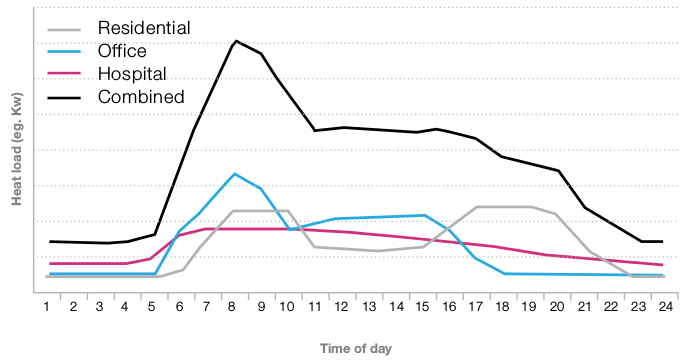
\includegraphics[width=0.5\linewidth]{mixLoad.png}
  \caption[Mixing Load Graph]{Mixing Load of Different Building
    Type~\cite{decentralHeatMap2011}}
  \label{fig:mixLoad}
\end{figure}

\subsection{More Detailed Description of Energy Behavior Supports
  Better Design}
A simple annual or monthly average cannot effectly represent the real
energy consumption behavior of an individual building and the whole
urban environment. In order to present this complicated behavior of
time-dependent energy demand, the time dimension is necessary.

This can be explained in a concrete example. Hospitals are usually
constant heat consumers with very stable heat demand throughout a year
(see \fref{fig:HG}), while a performance center is, on the other hand,
an occasional huge heat consumer with very high peak demand occuring
occasionally at event time and with almost zero demand in the
remaining time. It is reasonable to apply different energy planning
strategy for building groups involving one of these two types of
buildings. However, if time dimension is omitted, one has to choose
some aggregated description of the energy consumption of the two
building types, be it average, maximum, minimum or annual total. For
most cases, annual total demand is used for representing a building's
energy demand, especially in the case of District System design. With
this approach, the different energy usage pattern of a hospital and a
performance center might look the same, which results in a simplified
energy plan decision.

\subsection{Aggregation of Peak Value Becomes Tricky for Data with
  Time Variation}
One common mistake for sizing a district thermal energy system is to
add up the peak demand of each terminal users. Since the peak demand
of individual buildings do not occur at the same time, the end result
of summing up the peak demand at each end point exceeds the actual
total demand peak of the community. Hence with this approach, the
whole district system becomes excessively over-sized, which reduces
the whole system efficiency. A Dynamic Energy Map can reveal the
problem of such approaches by directly providing the aggregated
thermal energy and electricity demand for single buildings, building
sectors or the whole community. It allows a side by side comparison of
single building demand and aggregated demand and eliminates the
misunderstanding of the demand aggregation. With the direct
information of aggregated thermal energy and electricity demand, it
also assists actually sizing a district thermal energy system.



